\documentclass[10pt, a4paper,openany]{report} 
\usepackage{listings}
\usepackage{xcolor}
\usepackage[utf8]{inputenc}
\usepackage[spanish]{babel}
\addto\captionsspanish{\renewcommand{\contentsname}{Índice}}
\usepackage{graphicx}
\usepackage{amsmath}
\usepackage{amssymb}
\usepackage{amsfonts}
\usepackage{lipsum}
\usepackage[ left=2.54cm, right=2.54cm, top=2.54cm, bottom=2.54cm]{geometry}
\usepackage[hypertexnames=false]{hyperref}
\usepackage{titlesec}
\titleformat{\chapter}[display]
{\normalfont\bfseries}{}{0pt}{\Huge}
\titlespacing*{\chapter}{0pt}{-30pt}{10pt}
\setlength{\parindent}{1.25cm}
\lstdefinestyle{myStyle}{
  basicstyle=\small\ttfamily,
  columns=fullflexible,
  breaklines=true,
  breakatwhitespace=false,
  frame=single,
  aboveskip=10pt,
  belowskip=10pt,
  xleftmargin=10pt,
  xrightmargin=10pt,
  showstringspaces=false,
  commentstyle=\color{gray}\upshape
}



\begin{document}

\title{\Huge{Deltr0n}}
\author{Adrian Cespedes 202210088 \and Marcelo Chincha 202210092\and Lenin Chavez 202210090 \and Ibañes Flanklin Perez Muñoz 202020122}
\date{\null}

\maketitle
\tableofcontents
\chapter{Requisitos}
\label{cap:Requisitos}


\section{Introducción}
\label{sec:Introducción}

Un sistema basado en Deltron es una herramienta de gestión empresarial utilizada para supervisar las operaciones diarias de un importador y distribuidor mayorista de productos tecnológicos. Este sistema está pensado para facilitar la toma de decisiones, aumentar la eficacia operativa e impulsar el éxito financiero de la empresa.

El sistema está diseñado para gestionar una gran cantidad de datos, como el seguimiento de la cadena de suministro, la gestión de pedidos de compra y venta, la facturación y la contabilidad. El sistema también puede tener otras funciones, como la gestión de las relaciones con proveedores y clientes, la gestión de los recursos humanos y la creación y el análisis de informes.

Los usuarios de un sistema basado en Deltron pueden acceder a la información al instante y tomar decisiones basándose en los datos disponibles, ya que el sistema emplea una base de datos centralizada para albergar todos los datos de la empresa.

En resumen, un sistema basado en Deltron es una potente herramienta para la gestión empresarial en la importación y distribución de productos tecnológicos al por mayor, que ayuda a mejorar la eficacia operativa, la toma de decisiones y los resultados financieros de la empresa.


\section{Descripción general del problema/organización/empresa}
\label{sec:Descripción general del problema/organización/empresa}

El sistema de base de datos para una empresa como Deltron es una herramienta de gestión empresarial utilizada para supervisar las operaciones diarias de un importador y distribuidor mayorista de productos tecnológicos. Este sistema está pensado para facilitar la toma de decisiones, aumentar la eficacia operativa e impulsar el éxito financiero de la empresa por lo que será importante realizar un sistema de base de datos adecuados que soporte la gran cantidad de información y que permita realizar consultas en un tiempo esperado con un bajo coste.

\section{Necesidad/usos de la base de datos}
\label{sec:Necesidad/usos de la base de datos}

Es necesaria la base de datos porque es esencial para llevar registro de las compras, ventas, productos, inventario, empleados, etc. La base de datos debe poder administrar esta gran variedad de data.

\section{¿Cómo resuelva el problema hoy?}
\label{sec:¿Cómo resuelva el problema hoy?}

\subsection{¿Cómo se almacenan/procesan los datos hoy?}
\label{subsec:¿Cómo se almacenan/procesan los datos hoy?}

Los datos se almacenan en una base de datos relacional y se procesan con consultas SQL.

\subsection{Flujo de datos}
\label{subsec:Flujo de datos}

El flujo de datos de la empresa proviene de las empresas proveedoras de los productos, los clientes(personas no naturales) que compran los productos, los productos y su descripción, y los empleados que trabajan en la empresa.

\pagebreak

\section{Descripción detallada del sistema}
\label{sec:Descripción detallada del sistema}

\subsection{Objetos de información actuales }
\label{subsec:Objetos de información actuales }

La fuente de información son los clientes que compran los productos, los proveedores que venden los productos, los pedidos, los productos y su descripción, y los empleados que trabajan en la empresa. Tenemos 6 almacenes y almacenamos la información detallada de los pedidos, contando con que podríamos llegar a tener 10 000 pedidos diarios nuestro sistema de base de datos podría almacenar con facilidad 1 millón de datos al año, lo esperado es un aproximado de 4000 pedidos diarios y 400000 datos al año.

\subsection{Características y funcionalidades esperadas}
\label{subsec:Características y funcionalidades esperadas}

El sistema de base de datos esta relacionado a la gestión de pedidos de compra y venta, la facturación y la contabilidad. El sistema también puede tener otras funciones, como la gestión de las relaciones con proveedores y clientes.

\subsection{Tipos de usuarios existentes/necesarios}
\label{subsec:Tipos de usuarios existentes/necesarios}

\begin{itemize}
	\item Cliente: Realiza los pedidos de los productos y los compra, o en algún caso especial puede exigir un reembolso.
	\item Gerente: Administra a los empleados y los almacenes, puede realizar consultas sobre los pedidos, productos, empleados, etc.
	\item Fabricante: Provee los productos a la empresa.
\end{itemize}

\subsection{Tipos de consulta, actualizaciones }
\label{subsec:Tipos de consulta-actualizaciones }

\noindent Consultas que podrían hacer clientes y empleados:
\begin{itemize}
	\item Consultar el stock de un producto
	\item Consultar el precio de un producto en un almacén en una fecha
	\item Consultar el precio de un producto en un almacén en un rango de fechas
	\item Consultar cual ha sido el empleado que ha vendido más productos en un rango de fechas
	\item Consultar cual ha sido el cliente que ha pedido más productos en un rango de fechas
	\item Cual es el almacén que tiene más stock de un producto
	\item Comparar el precio entre productos en categorías similares
	\item Consultar el cliente que ha cancelado más pedidos
	\item Qué categoría tiene más productos
	\item Consultar características de cada producto
	\item Consultar que almacén tiene más ventas

\end{itemize}

\noindent Actualizaciones que podrían hacer clientes y empleados:
\begin{itemize}
	\item Actualizar el stock de un producto en un almacén
	\item Actualizar el precio de un producto en un almacén
	\item Los clientes pueden cambiar sus datos personales
	\item Se pueden cambiar los empleados en general
	\item Se pueden cambiar los datos de los productos
	\item Se pueden añadir almacenes

\end{itemize}

\subsection{Tamaño estimado de la base de datos}
\label{subsec:Tamaño estimado de la base de datos}

Para estimar el tamaño de la base de datos, consideramos las tablas del modelo relacional. De estas, tenemos algunas que son casi fijos, es decir, en un periodo se mantienen constantes, o aumentan, o disminuyen como los productos. Los pedidos crecerán cada día.


\begin{table}[h]
	\label{tab:Tamaño de las tablas}
	\begin{center}
		\begin{tabular}[c]{|c|c|c|}
			\hline
			\multicolumn{1}{|c|}{\textbf{Nombre de la tabla}}          &
			\multicolumn{1}{c}{\textbf{Longitud en Bytes por entrada}} &
			\multicolumn{1}{|c|}{\textbf{Longitud total por entrada}}                         \\
			\hline
			Cliente                                                    & 8+100+50+32+48 & 238 \\
			\hline
			Pedido                                                     & 8+8+8+3+3      & 30  \\
			\hline
			Pago                                                       & 8+8+4+32       & 52  \\
			\hline
			Reembolso                                                  & 8+8+8          & 24  \\
			\hline
			Despacho                                                   & 8+8+4          & 20  \\
			\hline
			Producto                                                   & 8+256+4+40     & 308 \\
			\hline
			Descuento                                                  & 8+4+4+4        & 20  \\
			\hline
			Fabricante                                                 & 40+50+50       & 140 \\
			\hline
			Categoria                                                  & 4+25+255       & 284 \\
			\hline
			almacén                                                    & 4+150          & 154 \\
			\hline
			Puerto                                                     & 4+150          & 154 \\
			\hline
			restock                                                    & 8+8+8+4        & 28  \\
			\hline
			Traslado\_Interno                                          & 4+4            & 8   \\
			\hline
			Persona                                                    & 8+12+50+50     & 120 \\
			\hline
			Recogedor\_Asignado                                        & 8+8            & 16  \\
			\hline
			Empleado                                                   & 8+12+255       & 275 \\
			\hline
			Atencion\_Cliente                                          & 8              & 8   \\
			\hline
			Almacenero                                                 & 8+4            & 12  \\
			\hline
			Inspectores                                                & 8              & 8   \\
			\hline
			Transportista                                              & 8              & 8   \\
			\hline
			Directivo                                                  & 8              & 8   \\
			\hline
			contiene\_P                                                & 8+8            & 16  \\
			\hline
			aplica                                                     & 8+8            & 16  \\
			\hline
			tiene                                                      & 4+8            & 12  \\
			\hline
			contiene\_T                                                & 8+4+4+4        & 20  \\
			\hline
			stock                                                      & 8+4+4          & 16  \\
			\hline
			g\_pedido                                                  & 40+8+4         & 52  \\
			\hline
			trae                                                       & 8+8+4+4+4      & 28  \\
			\hline
			monitoreo                                                  & 8+8+4          & 20  \\
			\hline
			encargado\_T                                               & 8+4+8+8        & 28  \\
			\hline
			encargado\_a                                               & 4+4+8          & 16  \\

			\hline
		\end{tabular}
	\end{center}
	\caption{Tamaño de las tablas}
\end{table}

\begin{table}[h]
	\label{tab:Tamaño de las tablas fijas}
	\begin{center}
		\begin{tabular}[c]{|c|c|c|c|}
			\hline
			\multicolumn{1}{|c|}{\textbf{Nombre de tabla}} &
			\multicolumn{1}{c}{\textbf{Tamaño en Bytes}}   &
			\multicolumn{1}{|c|}{\textbf{Datos estimados}} &
			\multicolumn{1}{|c|}{\textbf{Tamaño total en Bytes}}                           \\
			\hline
			Cliente                                        & 238 & 100 000   & 23 800 000  \\
			\hline
			Pedido                                         & 30  & 50 000    & 1 500 000   \\
			\hline
			Pago                                           & 52  & 45 000    & 2 340 000   \\
			\hline
			Reembolso                                      & 24  & 12 00     & 28 800      \\
			\hline
			Despacho                                       & 20  & 15 000    & 300 000     \\
			\hline
			Producto                                       & 308 & 1 000     & 308 000     \\
			\hline
			Descuento                                      & 20  & 650       & 13 000      \\
			\hline
			Fabricante                                     & 140 & 120       & 16 800      \\
			\hline
			Categoria                                      & 284 & 15        & 4260        \\
			\hline
			almacén                                        & 154 & 9         & 1386        \\
			\hline
			Puerto                                         & 154 & 12        & 1848        \\
			\hline
			restock                                        & 28  & 16        & 448         \\
			\hline
			Traslado\_Interno                              & 8   & 750       & 6000        \\
			\hline
			Persona                                        & 120 & 1 000 000 & 120 000 000 \\
			\hline
			Recogedor\_Asignado                            & 16  & 45 000    & 720 00      \\
			\hline
			Empleado                                       & 275 & 1000      & 275 000     \\
			\hline
			Atencion\_Cliente                              & 8   & 70        & 560         \\
			\hline
			Almacenero                                     & 12  & 400       & 4800        \\
			\hline
			Inspectores                                    & 8   & 40        & 320         \\
			\hline
			Transportista                                  & 8   & 190       & 1520        \\
			\hline
			Directivo                                      & 8   & 3         & 24          \\
			\hline
			contiene\_P                                    & 16  & 50 000    & 800 000     \\
			\hline
			aplica                                         & 16  & 30 000    & 480 000     \\
			\hline
			tiene                                          & 12  & 100 000   & 1 200 000   \\
			\hline
			contiene\_T                                    & 20  & 7 500     & 150 000     \\
			\hline
			stock                                          & 16  & 1000      & 16000       \\
			\hline
			g\_pedido                                      & 52  & 16        & 832         \\
			\hline
			trae                                           & 28  & 180       & 5040        \\
			\hline
			monitoreo                                      & 20  & 468       & 9 360       \\
			\hline
			encargado\_T                                   & 28  & 16        & 448         \\
			\hline
			encargado\_a                                   & 16  & 750       & 12 000      \\

			\hline
		\end{tabular}
	\end{center}
	\caption{Tamaño anual estimado de las tablas fijas}
\end{table}
\pagebreak



\section{Objetivos del proyecto}
\label{sec:Objetivos del proyecto}

\begin{itemize}
	\item Crear un sistema de base de datos para aquellas empresas que importen internacionalmente y distribuyan localmente
	\item Se espera facilitar el procesamiento de datos y que se pueda llevar un histórico adecuado de cada compra y venta
	\item Optimizar los tiempos de respuesta de la base de datos de manera que sea capaz de soportar
	      consultas complejas a pesar de su enorme cantidad de data.

\end{itemize}

\section{Referencias del proyecto}
\label{sec:Referencias del proyecto}

Este proyecto esta basado en la empresa Deltron S.A. y su descripción se encuentra en la introducción.

\section{Eventualidades}
\label{sec:Eventualidades}

\subsection{Problemas que pudieran encontrarse en el proyecto}
\label{subsec:Problemas que pudieran encontrarse en el proyecto}

Este apartado será llenado a medida que se vaya desarrollando el proyecto.

\subsection{Límites y alcances del proyecto}
\label{subsec:Límites y alcances del proyecto}

\begin{itemize}
	\item Alcances : \\ Este proyecto busca un alcance nacional, ya que los clientes solo pueden ser personas jurídicas en Perú.
	\item Límites : \\ Todos los datos solo pueden estar en inglés o español, y los reclamos pueden ser atendidos con muchas demoras.
\end{itemize}

\chapter{Modelo Entidad-Relación}
\label{cap:Modelo Entidad-Relación}

\section{Reglas semánticas}
\label{sec:Reglas semánticas}

\noindent En el diseño del modelo E-R se deben tomar en cuenta las siguientes reglas semánticas:
\begin{itemize}
	\item El cliente (empresa) se identifica por su razón social, RUC, correo electrónico, contraseña, número de teléfono.
	\item El cliente puede ser mayorista o minorista, se diferencia por que el mayorista tiene asignado un descuento por producto final.
	\item Se poseen 6 almacenes distribuidos a lo largo del país, estos se identifican por un único número en orden(de 1 a n) y se almacena su dirección en conjunto.
	\item Un cliente puede realizar 0 a n pedidos en el sistema. Los cuales son identificados a través de una ID única, el DNI de la persona a recibir, la fecha de generación, fecha límite de pago (derivado, se calcula 3 días a partir de la generación).
	\item Todos los pedidos pueden ser realizados por los clientes de manera virtual o presencial, en ambos se requiere de guardar el almacén donde se realizó dicho proceso y el agente que lo atendió (en caso sea virtual, este será “virtual”).
	\item Los descuentos y/o ofertas solo aplican a productos. Este necesita almacenar el código de promoción,la fecha de inicio y límite. También requiere una condición necesaria para aplicar el descuento.
	\item Todos los productos deben estar en al menos un almacén, y se necesita almacenar el monto de cuantas unidades respectivas hay.
	\item El producto tiene un id único, nombre, descripción, precio actual y su respectivo fabricante. Además los productos podemos clasificarlos en categorías. Y las categorías tienen un código, nombre.
	\item La compra solo se puede realizar con un pedido. Que requiere el monto total a pagar del pedido(con descuentos aplicados) y el almacén a recoger. También se deberá especificar la persona que recoge el pedido con su DNI.
	\item Para recoger el pedido cancelado, el cliente designa a una persona autorizada para recoger el pedido en el almacén respectivo. Es necesario guardar su DNI y un número de teléfono.
	\item Cada almacén recibe productos importados los cuales deben ser registrados por cada almacén respectivamente, donde se guarda la fecha de llegada de los productos al almacén, y los nuevos almacenados(Aunque sean nuevos siempre estarán en el sistema). Todo el “re stock” deberá tener como  mínimo un producto nuevo para el almacén.
	\item Para recibir más productos nuevos desde los fabricantes un directivo realiza un pedido de compra a cada uno de los fabricantes. Donde se detalla los productos a pedir, la fecha de realización, y el monto total de pago.
	\item Un fabricante se identifica a través de su nombre,país y su dominio de correo electrónico.
	\item El lugar donde se cargan los productos importados es el puerto marítimo(se importa mediante containers)  más cercano al respectivo almacén. Cada puerto se identifica con una dirección.
	\item Es posible que se tengan que trasladar uno o varios ítems entre inventario, cuyo proceso se llama traslado, este es parecido al re stock(identificación  por fecha) pero ocurre entre almacenes y se necesita almacenar el almacén de inicio y de destino, y productos trasladados.
	\item Se poseen ciertos empleados encargados de diferentes tareas, pero en como estos tienen DNI, números de teléfono y correo electrónico institucional:
	      \begin{itemize}
		      \item Almaceneros:Trabajan en la parte de la descarga en los almacenes. Se necesita su respectivo almacén de trabajo(solo puede ser 1)
		      \item Atención al cliente: Interactúan con el cliente. Estos autorizan la venta de cada pedido, y atienden a las personas asignadas a recoger.
		      \item Inspectores: Verifican la integridad de los almacenes para observar o informar cualquier anomalía.
		      \item Transportistas: Pueden trasladar diversos productos a diferentes almacenes.
		      \item Directivos: Tienen que realizar labores administrativas de alto nivel en toda la empresa. Como aprobar contratos y/o importaciones.

	      \end{itemize}
	\item Los inspectores realizan diferentes observaciones de los almacenes cada mes. Debido a que la parte corporativa de la empresa requiere reportes acerca del estado de los almacenes. En cada reporte se toma en cuenta al almacén que se inspeccionó, la fecha, y el código de inspección(se genera partir de la fecha e id del almacén). También  se debe almacenar los inspectores involucrados en dicha operación, que como mínimo, debió haber estado uno presente.

	\item En caso de que un producto esté defectuoso se puede realizar un trámite de reembolso, en el cual se devuelve el dinero al cliente por el producto a entregar. Para ello se necesita el código de la venta correspondiente al producto y los productos a rembolsar. Cabe aclarar que se puede devolver los productos en cualquier almacén disponible.
	\item La empresa tiene una política de productos defectuosos si han sido reembolsados se procederá a hacer un pedido a los fabricantes para que reemplace dicho componente. Este trámite requiere de una fecha , un código identificador y el fabricante al cual se hará el envío de dichos productos.

\end{itemize}
\section{Modelo Entidad-Relación}
\label{sec:Modelo Entidad-Relación}

En anexo



\section{Especificaciones y consideraciones sobre el modelo}
\label{sec:Especificaciones y consideraciones sobre el modelo}

\noindent \textbf{En esta sección se describirá el modelo relacional para explicarlo.}

\begin{enumerate}
	\item  Cliente:
	      \begin{itemize}
		      \item Especificaciones:
		            Guarda la información básica de un cliente, el cual debería ser una persona jurídica, el cual contiene RUC(llave primaria) y también se toma en cuenta
		            su razón social y numero de teléfono.
		      \item Consideraciones:
		            El RUC del cliente siempre sera diferente, esto permite a que pueda ser la llave candidata mas adecuada para la tabla. También el teléfono no es considerado multivariado
		            puesto a que se espera que un cliente tenga un único numero de teléfono para mantener el orden en las comunicaciones.
	      \end{itemize}

	\item  Pedido:
	      \begin{itemize}
		      \item Especificaciones:
		            Contiene datos acerca de los productos requeridos por los clientes, este contiene un ID como llave primaria y permite múltiples productos por pedido con los productos.
		      \item Consideraciones:
		            El pedido siempre esta relacionado con la entidad pago de forma débil, es decir, el pago solo existe para un pedido establecido anteriormente. También de relaciona de 1 a 1 con la entidad
		            despacho, lo que indica que este puede ser despachado una única vez.
	      \end{itemize}

	\item  Producto:
	      \begin{itemize}
		      \item Especificaciones:
		            Esta debe almacenar, como llave, un id de producto para poder diferenciarlos, un precio con un nombre y descripción(el cual llega a ser algo grande).
		      \item Consideraciones:
		            Siendo este una de las entidades mas importantes en todo el diagrama, puesto a que tiene muchas relaciones entre entidades diferentes. Consecuentemente el id es útil para poder diferenciar a los pedidos
		            no solo en casos de compra sino también en devoluciones.
	      \end{itemize}

	\item  Descuento:
	      \begin{itemize}
		      \item Especificaciones:
		            Tiene como llave primaria un ID, una fecha de inicio y fin, y también el porcentaje de reducción de precio.
		      \item Consideraciones:
		            En el diagrama se puede apreciar que un descuento puede ser aplicado a varios productos pero este solo puede aplicarse a un descuento activo. Esto permite a que no se puedan canjear
		            mas rebajas al mismo tiempo.
	      \end{itemize}


	\item  Fabricante:
	      \begin{itemize}
		      \item Especificaciones:
		            Requiere de nombre como llave primaria, país de origen y su dominio de correo privado.
		      \item Consideraciones:
		            La llave primaria, como nombre, es pertinente de usar puesto a que 2 empresas no deberían tener el mismo nombre, y por eso el nombre es una llave primaria.
	      \end{itemize}


	\item  Categoria:
	      \begin{itemize}
		      \item Especificaciones:
		            Contiene un ID como llave primaria y un nombre de la categoria.
		      \item Consideraciones:
		            Varios productos pueden poseen diversas categorías, esto es conveniente al usar una entidad como categoría puesto a que permite que todos los productos tengan los mismos tipos en común
	      \end{itemize}


	\item  Pago:
	      \begin{itemize}
		      \item Especificaciones:
		            Contiene un ID de venta, un monto asignado al pedido y el monto requiero a pagar
		      \item Consideraciones:
		            Como ya se menciono antes esta entidad es débil a pedido puesto a que solo existe uno para cada , aunque también puede ser conveniente usar el mismo pago
		            como método de rembolso en cada  productos defectuosos.
	      \end{itemize}

	\item  Reembolso:
	      \begin{itemize}
		      \item Especificaciones:
		            Solo contiene como llave primaria un ID de pedido de rembolso y la fecha.
		      \item Consideraciones:
		            Esta entidad es débil a pedido puesto a que solo existe uno para cada pedido,puesto a que solo hay un reembolso por pedido pagado.
	      \end{itemize}

	\item  Despacho:
	      \begin{itemize}
		      \item Especificaciones:
		            Posee una llave parcial indicando el nro de despacho, y también una fecha de despacho, como llave foránea primaria se tiene el ID de pedido.
		      \item Consideraciones:
		            El despacho solo puede ser realizado una vez, es por ello que se relaciona con la entidad pedido de forma débil, puesto a que el despacho solo existe para un pedido.
	      \end{itemize}


	\item  Almacen:
	      \begin{itemize}
		      \item Especificaciones:
		            Contiene un Nro de almacén el cual es una llave primaria para poder diferenciarlas, también posee una dirección.
		      \item Consideraciones:
		            Esta entidad permite el almacenamiento de productos.
	      \end{itemize}

	\item Traslado\_Interno :
	      \begin{itemize}
		      \item Especificaciones:
		            Es una entidad débil de almacén, el cual posee una llave parcial: almacén\_destino.
		      \item Consideraciones:
		            Esta entidad permite el traslado de productos entre almacenes, aunque esto puede ser tedioso al momento de buscar un producto en especifico.
	      \end{itemize}


	\item  Restock:
	      \begin{itemize}
		      \item Especificaciones:
		            Contiene un ID único, el cual es una llave parcial, y también posee una fecha de re stock, esta relacionado de manera débil con almacén y Puerto, añadiendo 2 llaves primarias foráneas.
		      \item Consideraciones:
		            Esta entidad permite el re stock de productos en un almacén, desde un puerto especifico hasta un almacén.
	      \end{itemize}

	\item  Puerto:
	      \begin{itemize}
		      \item Especificaciones:
		            Solo tiene un ID como llave primaria y una dirección.
		      \item Consideraciones:
		            Los productos nuevos llegan a esta entidad, es por ello que la entidad re stock depende de este.
	      \end{itemize}


	\item Persona:
	      \begin{itemize}
		      \item Especificaciones:
		            Se le atribuye: un DNI y teléfono como como una súper llave, un nombre, apellido.
		      \item Consideraciones:
		            Esta entidad almacena los datos de todos las personas involucradas activamente en el sistema como los empleados, etc.
	      \end{itemize}

	\item  Empleado:
	      \begin{itemize}
		      \item Especificaciones:
		            Es una subclase de la entidad persona, aunque se le añade el correo institucional de la empresa
		      \item Consideraciones:
		            Esta entidad almacena los datos de todos los empleados de la empresa, es posible describir mas tipos de empleados.
	      \end{itemize}

	\item  Recogedor asignado:
	      \begin{itemize}
		      \item Especificaciones:
		            No posee diferencias con la entidad persona.
		      \item Consideraciones:
		            Esta entidad se relaciona con la entidad despacho, puesto a que el cliente asignada a  una persona respectiva para recoger sus productos.
	      \end{itemize}

	\item Atencion al cliente:
	      \begin{itemize}
		      \item Especificaciones:
		            No posee diferencias con la entidad empleado.
		      \item Consideraciones:
		            Solo es relacionada con la entidad despacho, para poder realizar la constancia del respectivo despacho.
	      \end{itemize}

	\item Almacenero:
	      \begin{itemize}
		      \item Especificaciones:
		            No posee diferencias con la entidad empleado.
		      \item Consideraciones:
		            Encargado de  trabajar en 1 almacén en especifico.
	      \end{itemize}

	\item Inspector:
	      \begin{itemize}
		      \item Especificaciones:
		            No posee diferencias con la entidad empleado.
		      \item Consideraciones:
		            Esta relacionado a varios almacenes, puesto a que realiza varias inspecciones en diferentes almacenes validos.
	      \end{itemize}

	\item Transportista:
	      \begin{itemize}
		      \item Especificaciones:
		            No posee diferencias con la entidad empleado.
		      \item Consideraciones:
		            Puede realizar 2 tipos de viajes diferentes, la de re stock y la de traslado. Ambas lo relacionan con un almacén de destino.
	      \end{itemize}

	\item Directivo:
	      \begin{itemize}
		      \item Especificaciones:
		            No posee diferencias con la entidad empleado.
		      \item Consideraciones:
		            Permite autorizar los pedidos de importación, relacionándose con los fabricantes pertinentes y solicitando los productos a ser importados.
	      \end{itemize}
\end{enumerate}


\chapter{Modelo Relacional} % (fold)
\label{chap:Modelo Relacional}

% chapter Modelo Relacional (end)
\section{Modelo Relacional} % (fold)
\label{sec:Modelo Relacional}

\lstinputlisting{./mR.txt}




% section Modelo Relacional (end)
\section{Especificaciones de transformación} % (fold)
\label{sec:Especifiaciones de transformación}

% section Especifiaciones de transformación (end)

\subsection{Entidades} % (fold)
\label{sub:Entidades}


\begin{itemize}
	\item Cliente: Esta entidad su llave primaria es el RUC, tiene como atributos como razón social, contraseña Email, teléfono.
	\item Pedido: Esta entidad tiene un solo atributo ID que es su llave primaria. Absorbe F\_Creacion y F\_Limite.
	\item Producto: Su llave primaria que es ID y tiene como atributo nombre, precio y descripción.
	\item Descuento: El descuento tiene una llave primaria que es el ID y atributos  F\_inicio, F\_final y porcentaje.
	\item Categoría: Esta entidad tiene como atributos nombre y llave primaria de ID.
	\item Almacén:Tiene como atributos de dirección y  llave primaria Nro.
	\item Puerto: La entidad puerto tiene como atributos de dirección y llave primaria de ID.

	\item Fabricante: Tiene como llave primaria Nombre y atributos Pais y Dominio de correo.
\end{itemize}
% subsection Entidades (end)
\subsection{Entidades débiles} % (fold)
\label{sub:Entidades débiles}
\begin{itemize}
	\item Despacho:Es entidad débil de pedido, ya que solo existe en el contexto de pedido. Su llave primaria lo conforma el id del pedido, número de despacho. Sin embargo, tiene atributos de fecha.
	\item Pago:Es entidad débil de pedido, ya que solo existe en el contexto de pedido. Su llave primaria lo conforma el id del pedido, ID de sí mismo, y atributos como monto, método.
	\item Reembolso:Es una entidad débil de monto, ya que solo puede existir en el contexto de pago. Su llave primaria lo conforma el id del pedido y el ID de sí mismo con atributo Fecha.
	\item Traslado interno:Es entidad débil de almacén.Su llave primaria lo  conforma almacén       destino y Nro almacén con atributo Fecha.
	\item Restock: Es una entidad débil de Almacén y Puerto, ya que existe en el contexto de los 2 entidades. Su llave primaria es ID, Nro\_Almacen, ID\_Puerto. y el otro atributo es la Fecha.

\end{itemize}

% subsection Entidades débiles (end)

\subsection{Entidades superclase/subclases} % (fold)
\label{sub:Entidades superclase/subclases}
\begin{itemize}
	\item Superclase Persona:Esta superclase cuenta con los atributos DNI, nombre, apellidos y teléfono.Las llaves primarias son el DNI y el teléfono y hay 2 entidades que heredan esta clase. No hay solapamiento ni cobertura.
	      \begin{itemize}
		      \item Subclases:
		      \item Recogedor Asignado: El recogedor asignado hereda los atributos de la clase persona.
		      \item Empleado: Hereda los atributos de la clase persona y además tiene un atributo que es el correo institucional.
	      \end{itemize}
	\item Superclase Empleado: Esta superclases cuenta con los atributos de correo institucional. La llave primaria es Persona.DNI y esta entidad heredan 5 entidades. No hay cobertura ni solapamiento.
	      \begin{itemize}
		      \item Subclases:
		      \item Atención al cliente: Supervisa el despacho de los pedidos pagados.
		      \item Inspectores: Monitorizan los almacenes.
		      \item Transportistas: Encargados de los traslados internos y llegados del puerto.
		      \item Directivo: Encargado de realizar pedidos a los fabricantes.
	      \end{itemize}


\end{itemize}

% subsection Entidades superclase/subclases (end)

\subsection{Relaciones binarias} % (fold)
\label{sub:Relaciones binarias}

\begin{itemize}
  \item Trabaja: La relación se da entre cliente y recogedor asignado. El cliente tiene una multiplicidad de 0:n ya que puede tener varios asignados para recoger. El Recogedor asignado tiene una multiplicidad de 1:1, ya que solo puede trabajar para un cliente(Empresa).

\item Realiza\_Pedido: Esta relación tiene como atributos F\_creación, F\_Limite. Y la relación se da entre las entidades Cliente y Pedido. La multiplicidad de Cliente(Empresa) es de 0:n, ya que puede realizar  de 0 a n pedidos. La multiplicidad de Pedido es de exactamente 1:1, ya que cada pedido solo puede ser realizado por un cliente.

\item Asignado: La relación entre las entidades de Pedido y Recogedor asignado. El pedido tiene una multiplicidad de 1:1, ya que cada pedido solo puede tener un recogedor asignado. La multiplicidad de recogedor asignado es de 0:n, ya puede ser asignado a varios pedidos.
 
\item Contiene\_P: Esta relación se da entre Pedido y Producto. La multiplicidad de Pedido es de 1:n, que en un pedido puede tener 1:n productos; y la multiplicidad de Producto es de 1:n, cada productos puede ser pedidos de 1 a n pedidos.
\item Aplica: Esta relación se da entre las entidades Producto y Descuento. La multiplicidad de  Producto es 0:1, ya que el producto solo puede tener 0 o 1 un descuento. La multiplicidad de Descuento es de 0:n, ya que el descuento se puede aplicar a varios productos.
\item Fabricado por: Esta relación se da entre las entidades Producto y Fabricante. La multiplicidad de Producto es de 1:1, ya que puede ser fabricado por exactamente por un fabricante. La multiplicidad de Fabricante es de 0:n, ya que puede fabricar de 0:n productos. 
\item Tiene: Esta relación se da entre Producto y Categoria. Ambas multiplicidades son de 1:n; ya que, Producto tiene por lo menos una Categoria y este último pertenece a más de un Producto.
\item Stock: Esta relación se da entre Producto y almacén. La multiplicidad de  producto es de 1:n, ya que puede haber de 1:n stocks en el almacén. La multiplicidad de Almacén es de  0:n, ya que puede haber de 0 a n cantidades de cada producto.

\item Contiene\_T: Relación entre Producto y Traslado\_Interno. La multiplicidad de Producto es 0:n porque puede o no ser contenido en un Stock. Traslado\_Interno es 1:n; ya que, este contiene por lo menos un Producto.
\item Trae: Relación entre Producto y re stock. La multiplicidad de Producto es 0:n porque puede o no ser traído para un re stock. Re stock es 1:n; ya que, este contiene por lo menos un Producto.

\item Trabaja: Relación entre Almacenero y Almacén. La multiplicidad de Almacenero es 1:1; ya que este trabaja en exactamente un Almacén. Y del otro lado, 1:n; ya que se tiene por lo menos un Almacenero.
\item Monitoreo: Esta relación se da entre las entidades Inspector y Almacenero. La multiplicidad de Almacén es de 1:n, ya que puede ser monitorizado  por 1:n almaceneros en diferentes fechas. La multiplicidad de  Almacenero es de 1:n, ya que un Almacenero puede monitorizar de 1 a n almacenes en diferentes fechas.
\item Encargado\_T: Relación entre re stock y Transportista. Ambas tienen multiplicidad 1:n porque en un re stock participan por lo menos un Transportista y este último puede participar en mínimo un re stock.
\item Encargado\_A: Relación entre Traslado\_Interno y Transportista. Ambas tienen multiplicidad 1:n porque en un Traslado\_Interno participan por lo menos un Transportista y este último puede participar en mínimo un Traslado\_Interno .

\end{itemize}

% subsection Relaciones binarias (end)

\subsection{Relaciones ternarias} % (fold)
\label{sub:Relaciones ternarias}

\begin{itemize}
  \item G\_Pedido: Esta relación se da entre las relaciones de Fabricante, Producto y Directivo. La multiplicidad de Fabricante es de 0:n, ya que puede haber de 0 a n pedidos de producto y Directivo. La multiplicidad de Producto es de 1:n, porque hay por lo menos uno de ellos en el G\_Pedido y la multiplicidad de Directivo es de 0:n; ya que, puede realizar o no pedidos.
\end{itemize}

\begin{itemize}
  \item 
\end{itemize}



% subsection Relaciones ternarias (end)
\section{Diccionario de datos} % (fold)
\label{sec:Diccionario de datos}

\begin{table}[h]
\centering
\begin{tabular}{|l|p{2cm}|p{0.5cm}|p{0.5cm}|p{3cm}|}
\hline
\textbf{Nombre} &
\textbf{Dominio} &
\textbf{PK} &
\textbf{FK} &
\textbf{Descripción} \\
\hline
RUC & bigint & x & & Registro Único de Contribuyentes del cliente \\
\hline
email & varchar(100) & & & Correo electrónico del cliente \\
\hline
razon\_social & varchar(50) & & & Razón social del cliente \\
\hline
contrasenha & varchar(32) & & & Contraseña del cliente \\
\hline
teléfono & varchar(12) & & & Teléfono del cliente \\
\hline
\end{tabular}
\caption{Tabla Cliente}
\end{table}


\begin{table}[h]
	\centering
	\begin{tabular}{|l|p{1.5cm}|p{0.5cm}|p{0.5cm}|p{3cm}|}
		\hline
		\textbf{Nombre}         &
		\textbf{Dominio}        &
		\textbf{PK}             &
		\textbf{FK}             &
		\textbf{Descripción}                                                                                          \\
		\hline
		id                      & bigint & x &   & Identificador único del pedido                                     \\
		\hline
		Cliente.Ruc             & bigint &   & x & Registro Único de Contribuyentes del cliente que realizó el pedido \\
		\hline
		Recogedor\_Asignado.DNI & bigint &   & x & Documento Nacional de Identidad del recogedor asignado al pedido   \\
		\hline
		f\_creacion             & date   &   &   & Fecha de creación del pedido                                       \\
		\hline
		f\_limite               & date   &   &   & Fecha límite de pago del pedido                                    \\
		\hline
	\end{tabular}
	\caption{Tabla Pedido}
\end{table}


\begin{table}[h]
	\centering
	\begin{tabular}{|l|p{1.5cm}|p{0.5cm}|p{0.5cm}|p{3cm}|}
		\hline
		\textbf{Nombre} & \textbf{Dominio} & \textbf{PK} & \textbf{FK} & \textbf{Descripción}                                       \\
		\hline
		id              & bigint           & x           & x           & Identificador único del pago asociado a un pedido          \\
		\hline
		Pedido.id       & bigint           & x            & x           & Identificador único del pedido asociado al pago            \\
		\hline
		monto           & float            &             &             & Monto del pago realizado                                   \\
		\hline
		metodo          & varchar(32)      &             &             & Método de pago utilizado (por ejemplo, tarjeta de crédito) \\
		\hline
	\end{tabular}
	\caption{Tabla Pago}
\end{table}

\begin{table}[h]
	\centering
	\begin{tabular}{|l|p{1.5cm}|p{0.5cm}|p{0.5cm}|p{3cm}|}
		\hline
		\textbf{Nombre} & \textbf{Dominio} & \textbf{PK} & \textbf{FK} & \textbf{Descripción}                                                  \\
		\hline
		id              & bigint           & x           &             & Identificador único del reembolso                                     \\
		\hline
		Pago.id         & bigint           & x            & x           & Identificador único del pago asociado al reembolso                    \\
		\hline
		Pedido.id       & bigint           & x            & x           & Identificador único del pedido asociado al pago asociado al reembolso \\
		\hline
	\end{tabular}
	\caption{Tabla Reembolso}
\end{table}

\begin{table}[h]
	\centering
	\begin{tabular}{|l|p{1.5cm}|p{0.5cm}|p{0.5cm}|p{3cm}|}
		\hline
		\textbf{Nombre} & \textbf{Dominio} & \textbf{PK} & \textbf{FK} & \textbf{Descripción}                                \\
		\hline
		nro\_Despacho   & bigInt           & x         &  & Número único identificador del despacho             \\
		\hline
		Pedido.id       & bigInt           &     x       & x& Identificador único del pedido asociado al despacho \\
		\hline
		fecha           & date             &           &  & Fecha en que se realizó el despacho                 \\
		\hline
	\end{tabular}
	\caption{Tabla Despacho}
\end{table}

\begin{table}[h]
	\centering
	\begin{tabular}{|l|p{2cm}|p{0.5cm}|p{0.5cm}|p{3cm}|}
		\hline
		\textbf{Nombre}   & \textbf{Dominio} & \textbf{PK}& \textbf{FK} & \textbf{Descripción}               \\
		\hline
		id                & bigInt           & x        &   & Identificador único del producto   \\
		\hline
		nombre            & varchar(256)     &          &   & Nombre del producto                \\
		\hline
		precio            & float            &          &   & Precio del producto                \\
		\hline
		Fabricante.nombre & varchar(40)      &          &x   & Nombre del fabricante del producto \\
		\hline
	\end{tabular}
	\caption{Tabla Producto}
\end{table}

\begin{table}[h]
	\centering
	\begin{tabular}{|l|p{1.5cm}|p{0.5cm}|p{3cm}|}
		\hline
		\textbf{Nombre} & \textbf{Dominio} & \textbf{PK} & \textbf{Descripción}              \\
		\hline
		id              & bigInt           & x           & Identificador único del descuento \\
		\hline
		F\_inicio       & date             &             & Fecha de inicio del descuento     \\
		\hline
		F\_fin          & date             &             & Fecha de fin del descuento        \\
		\hline
		porcentaje      & float            &             & Porcentaje de descuento aplicado  \\
		\hline
	\end{tabular}
	\caption{Tabla Descuento}
\end{table}

\begin{table}[h]
\centering
\begin{tabular}{|l|p{2cm}|p{0.5cm}|p{0.5cm}|p{3cm}|}
\hline
\textbf{Nombre} &
\textbf{Dominio} &
\textbf{PK} &
\textbf{FK} &
\textbf{Descripción} \\
\hline
nombre & varchar(40) & x & & Nombre del fabricante \\
\hline
pais & varchar(50) & & & País de origen del fabricante \\
\hline
dominio\_correo & varchar(50) & & & Dominio de correo electrónico del fabricante \\
\hline
\end{tabular}
\caption{Tabla Fabricante}
\end{table}

\begin{table}[h]
\centering
\begin{tabular}{|l|p{2cm}|p{0.5cm}|p{0.5cm}|p{3cm}|}
\hline
\textbf{Nombre} & \textbf{Dominio} & \textbf{PK} & \textbf{FK} & \textbf{Descripción} \\
\hline
id & int & x & & Identificador único de la categoría \\
\hline
nombre & varchar(25) & & & Nombre de la categoría \\
\hline
descripcion & varchar(255) & & & Descripción detallada de la categoría \\
\hline
\end{tabular}
\caption{Tabla Categoria}
\end{table}

\begin{table}[h]
\centering
\begin{tabular}{|l|p{2cm}|p{0.5cm}|p{0.5cm}|p{3cm}|}
\hline
\textbf{Nombre} & \textbf{Dominio} & \textbf{PK} & \textbf{FK} & \textbf{Descripción} \\
\hline
Nro & int & x & & Número de identificación del almacén \\
\hline
dirección & varchar(150) & & & Dirección del almacén \\
\hline
\end{tabular}
\caption{Tabla almacén}
\end{table}

\begin{table}[h]
\centering
\begin{tabular}{|l|p{2cm}|p{0.5cm}|p{0.5cm}|p{3cm}|}
\hline
\textbf{Nombre} & \textbf{Dominio} & \textbf{PK} & \textbf{FK} & \textbf{Descripción} \\
\hline
id & int & x & & Identificador único del puerto \\
\hline
dirección & varchar(150) & & & Dirección del puerto \\
\hline
\end{tabular}
\caption{Tabla Puerto}
\end{table}

\begin{table}[h]
\centering
\begin{tabular}{|l|p{1.5cm}|p{0.5cm}|p{0.5cm}|p{3cm}|}
\hline
\textbf{Nombre} &
\textbf{Dominio} &
\textbf{PK} &
\textbf{FK} &
\textbf{Descripción} \\
\hline
id & bigint & x & & Identificador único del re stock \\
\hline
almacén.id & bigint & x& x & Identificador del almacén que recibe el re stock \\
\hline
Puerto.id & bigint & x& x & Identificador del puerto del cual proviene la mercancía restockeada \\
\hline
fecha & date & & & Fecha en que se realizó el re stock \\
\hline
\end{tabular}
\caption{Tabla re stock}
\end{table}

\begin{table}[h]
\centering
\begin{tabular}{|l|p{1.5cm}|p{0.5cm}|p{0.5cm}|p{3cm}|}
\hline
\textbf{Nombre} &
\textbf{Dominio} &
\textbf{PK} &
\textbf{FK} &
\textbf{Descripción} \\
\hline
almacén\_destino & int & x &  & Identificador del almacén de destino del traslado interno \\
\hline
almacén.nro & int &x & x & Identificador del almacén de origen del traslado interno \\
\hline
\end{tabular}
\caption{Tabla Traslado\_Interno}
\end{table}

\begin{table}[h]
\centering
\begin{tabular}{|l|p{1.8cm}|p{0.5cm}|p{0.5cm}|p{3cm}|}
\hline
\textbf{Nombre} &
\textbf{Dominio} &
\textbf{PK} &
\textbf{FK} &
\textbf{Descripción} \\
\hline
DNI & bigint & x & & Documento Nacional de Identidad de la persona \\
\hline
teléfono & varchar(12) & & & Número de teléfono de la persona \\
\hline
nombre & varchar(50) & & & Nombre de la persona \\
\hline
apellido & varchar(50) & & & Apellido de la persona \\
\hline
\end{tabular}
\caption{Tabla Persona}
\end{table}
\begin{table}[h]
\centering
\begin{tabular}{|l|p{1.5cm}|p{0.5cm}|p{0.5cm}|p{3cm}|}
\hline
\textbf{Nombre} & \textbf{Dominio} & \textbf{PK} & \textbf{FK} & \textbf{Descripción} \\
\hline
dni & bigInt & x & & Documento Nacional de Identidad del recogedor \\
\hline
RUC & bigInt & & x & Registro Único de Contribuyentes del cliente \\
\hline
\end{tabular}
\caption{Tabla Recogedor\_Asignado}
\end{table}


\begin{table}[h]
\centering
\begin{tabular}{|l|p{2cm}|p{0.5cm}|p{0.5cm}|p{3cm}|}
\hline
\textbf{Nombre} & \textbf{Dominio} & \textbf{PK} & \textbf{FK} & \textbf{Descripción} \\
\hline
DNI & bigInt & x & & Documento Nacional de Identidad del empleado \\
\hline
teléfono & varchar(12) & & & Número de teléfono del empleado \\
\hline
correo\_institucional & varchar(255) & & & Correo electrónico institucional del empleado \\
\hline
\end{tabular}
\caption{Tabla Empleado}
\end{table}

\begin{table}[h]
\centering
\begin{tabular}{|l|p{1.5cm}|p{0.5cm}|p{0.5cm}|p{3cm}|}
\hline
\textbf{Nombre} & \textbf{Dominio} & \textbf{PK} & \textbf{FK} & \textbf{Descripción} \\
\hline
dni & bigInt & x & x & Documento Nacional de Identidad del empleado \\
\hline
\end{tabular}
\caption{Tabla Atencion\_Cliente}
\end{table} 

\begin{table}[h]
\centering
\begin{tabular}{|l|p{1.5cm}|p{0.5cm}|p{0.5cm}|p{3cm}|}
\hline
\textbf{Nombre} & \textbf{Dominio} & \textbf{PK} & \textbf{FK} & \textbf{Descripción} \\
\hline
Empleado.dni & bigInt &x & x & Documento Nacional de Identidad del empleado \\
\hline
almacén.nro & int & & x & Número del almacén donde trabaja el almacenero \\
\hline
\end{tabular}
\caption{Tabla Almacenero}
\end{table}

\begin{table}[h]
\centering
\begin{tabular}{|l|c|}
\hline
\textbf{Nombre} & \textbf{Dominio} \\
\hline
dni & bigInt \\
\hline
\end{tabular}
\caption{Tabla Inspectores}
\end{table}

\begin{table}[h]
\centering
\begin{tabular}{|l|c|}
\hline
\textbf{Nombre} & \textbf{Dominio} \\
\hline
dni & bigInt \\
\hline
\end{tabular}
\caption{Tabla Transportista}
\end{table}

\begin{table}[h]
\centering
\begin{tabular}{|l|c|}
\hline
\textbf{Nombre} & \textbf{Dominio} \\
\hline
dni & bigInt\\
\hline
\end{tabular}
\caption{Tabla Directivo}
\end{table}

\begin{table}[h]
\centering
\begin{tabular}{|l|c|c|}
\hline
\textbf{Nombre} & \textbf{Dominio} & \textbf{PK/FK} \\
\hline
Producto.Id & bigInt & PK \\
\hline
Pedido.id & bigInt & FK \\
\hline
\end{tabular}
\caption{Tabla contiene\_P}
\end{table}

\begin{table}[h]
\centering
\begin{tabular}{|l|c|c|}
\hline
\textbf{Nombre} & \textbf{Dominio} & \textbf{PK/FK} \\
\hline
Producto.id & bigInt & PK/FK \\
\hline
Descuento.id & bigInt & PK/FK \\
\hline
\end{tabular}
\caption{Tabla aplica}
\end{table}

\begin{table}[h]
\centering
\begin{tabular}{|l|c|c|}
\hline
\textbf{Nombre} & \textbf{Dominio} & \textbf{PK/FK} \\
\hline
Producto.id & bigInt & PK/FK \\
\hline
Categoria.id & int & PK/FK \\
\hline
\end{tabular}
\caption{Tabla tiene}
\end{table}

\begin{table}[h]
\centering
\begin{tabular}{|l|c|c|c|}
\hline
\textbf{Nombre} & \textbf{Dominio} & \textbf{PK} & \textbf{FK} \\
\hline
Producto.id & bigInt & x &x \\
\hline
Traslado\_interno.almacén\_destino & int & x & x\\
\hline
almacén.nro & int & x& x \\
\hline
\end{tabular}
\caption{Tabla contiene\_T}
\end{table}

\begin{table}[h]
\centering
\begin{tabular}{|l|p{1.5cm}|p{0.5cm}|p{0.5cm}|p{3cm}|}
\hline
\textbf{Nombre} &
\textbf{Dominio} &
\textbf{PK} &
\textbf{FK} &
\textbf{Descripción} \\
\hline
Producto.id & bigint & x &x & Identificador único del producto \\
\hline
almacén.id & int & x & x & Identificador único del almacén \\
\hline
cantidad & int & & & Cantidad de productos en el almacén \\
\hline
\end{tabular}
\caption{Tabla Stock}
\end{table} 

\begin{table}[h]
\centering
\begin{tabular}{|l|p{1.5cm}|p{0.5cm}|p{0.5cm}|p{3cm}|}
\hline
\textbf{Nombre} &
\textbf{Dominio} &
\textbf{PK} &
\textbf{FK} &
\textbf{Descripción} \\
\hline
Fabricante.Nombre & varchar(40) & x & x & Nombre del fabricante del producto \\
\hline
Directivo.DNI & bigint & x& x & Documento Nacional de Identidad del gerente que realizó el pedido \\
\hline
fecha & date & & & Fecha en que se realizó el pedido \\
\hline
\end{tabular}
\caption{Tabla G\_Pedido}
\end{table}

\begin{table}[h]
\centering
\begin{tabular}{|l|p{1.5cm}|p{0.5cm}|p{0.5cm}|p{3cm}|}
\hline
\textbf{Nombre} &
\textbf{Dominio} &
\textbf{PK} &
\textbf{FK} &
\textbf{Descripción} \\
\hline
Producto.id & bigint & x & x & Identificador único del producto que se va a traer \\
\hline
restock.id & bigint & x & x & Identificador único del re stock al que pertenece el producto \\
\hline
almacén.Nro & int & & x & Número identificador del almacén desde donde se va a traer el producto \\
\hline
Puerto.id & int & & x & Identificador único del puerto de destino \\
\hline
Cantidad & int & & & Cantidad de productos que se van a traer \\
\hline
\end{tabular}
\caption{Tabla Trae}
\end{table}


\begin{table}[h]
\centering
\begin{tabular}{|l|p{1.5cm}|p{0.5cm}|p{0.5cm}|p{3cm}|}
\hline
\textbf{Nombre} &
\textbf{Dominio} &
\textbf{PK} &
\textbf{FK} &
\textbf{Descripción} \\
\hline
Inspectores.DNI & bigint & x & x & Documento Nacional de Identidad del inspector encargado del monitoreo \\
\hline
almacén.Nro & int & x & x & Número de identificación del almacén monitorizado \\
\hline
fecha & date & & & Fecha en que se realizó el monitoreo \\
\hline
\end{tabular}
\caption{Tabla Monitoreo}
\end{table}

\begin{table}[h]
\centering
\begin{tabular}{|l|p{1.5cm}|p{0.5cm}|p{0.5cm}|p{3cm}|}
\hline
\textbf{Nombre} &
\textbf{Dominio} &
\textbf{PK} &
\textbf{FK} &
\textbf{Descripción} \\
\hline
restock.id & bigint & x & x & Identificador único del re stock \\
\hline
almacén.Nro & int &x & x & Número de identificación del almacén de origen del re stock \\
\hline
Puerto.id & int & x& x & Identificador único del puerto donde se recibió el envío del re stock \\
\hline
Transportista.DNI & bigint &x& x & Documento Nacional de Identidad del transportista encargado de entregar el envío \\
\hline
\end{tabular}
\caption{Tabla Encargado\_T}
\end{table}

\begin{table}[h]
\centering
\begin{tabular}{|l|p{1.5cm}|p{0.5cm}|p{0.5cm}|p{3cm}|}
\hline
\textbf{Nombre} &
\textbf{Dominio} &
\textbf{PK} &
\textbf{FK} &
\textbf{Descripción} \\
\hline
Traslado\_Interno.almacén\_destino & int & x & x & Número de identificación del almacén de destino del traslado interno \\
\hline
almacén.Nro & int & x & x & Número de identificación del almacén de origen del traslado interno \\
\hline
Transportista.DNI & bigint & x & x & Documento Nacional de Identidad del transportista encargado del traslado \\
\hline
\end{tabular}
\caption{Tabla Encargado\_a}
\end{table}
% section Diccionario de datos (end)

\chapter{Implementación de la base de datos} % (fold)
\label{chap:Implementación de la base de datos}

% chapter Implementación de la base de datos (end)


\chapter{ANEXOS} % (fold)
\label{chap:ANEXOS}
\vspace {0.5cm}
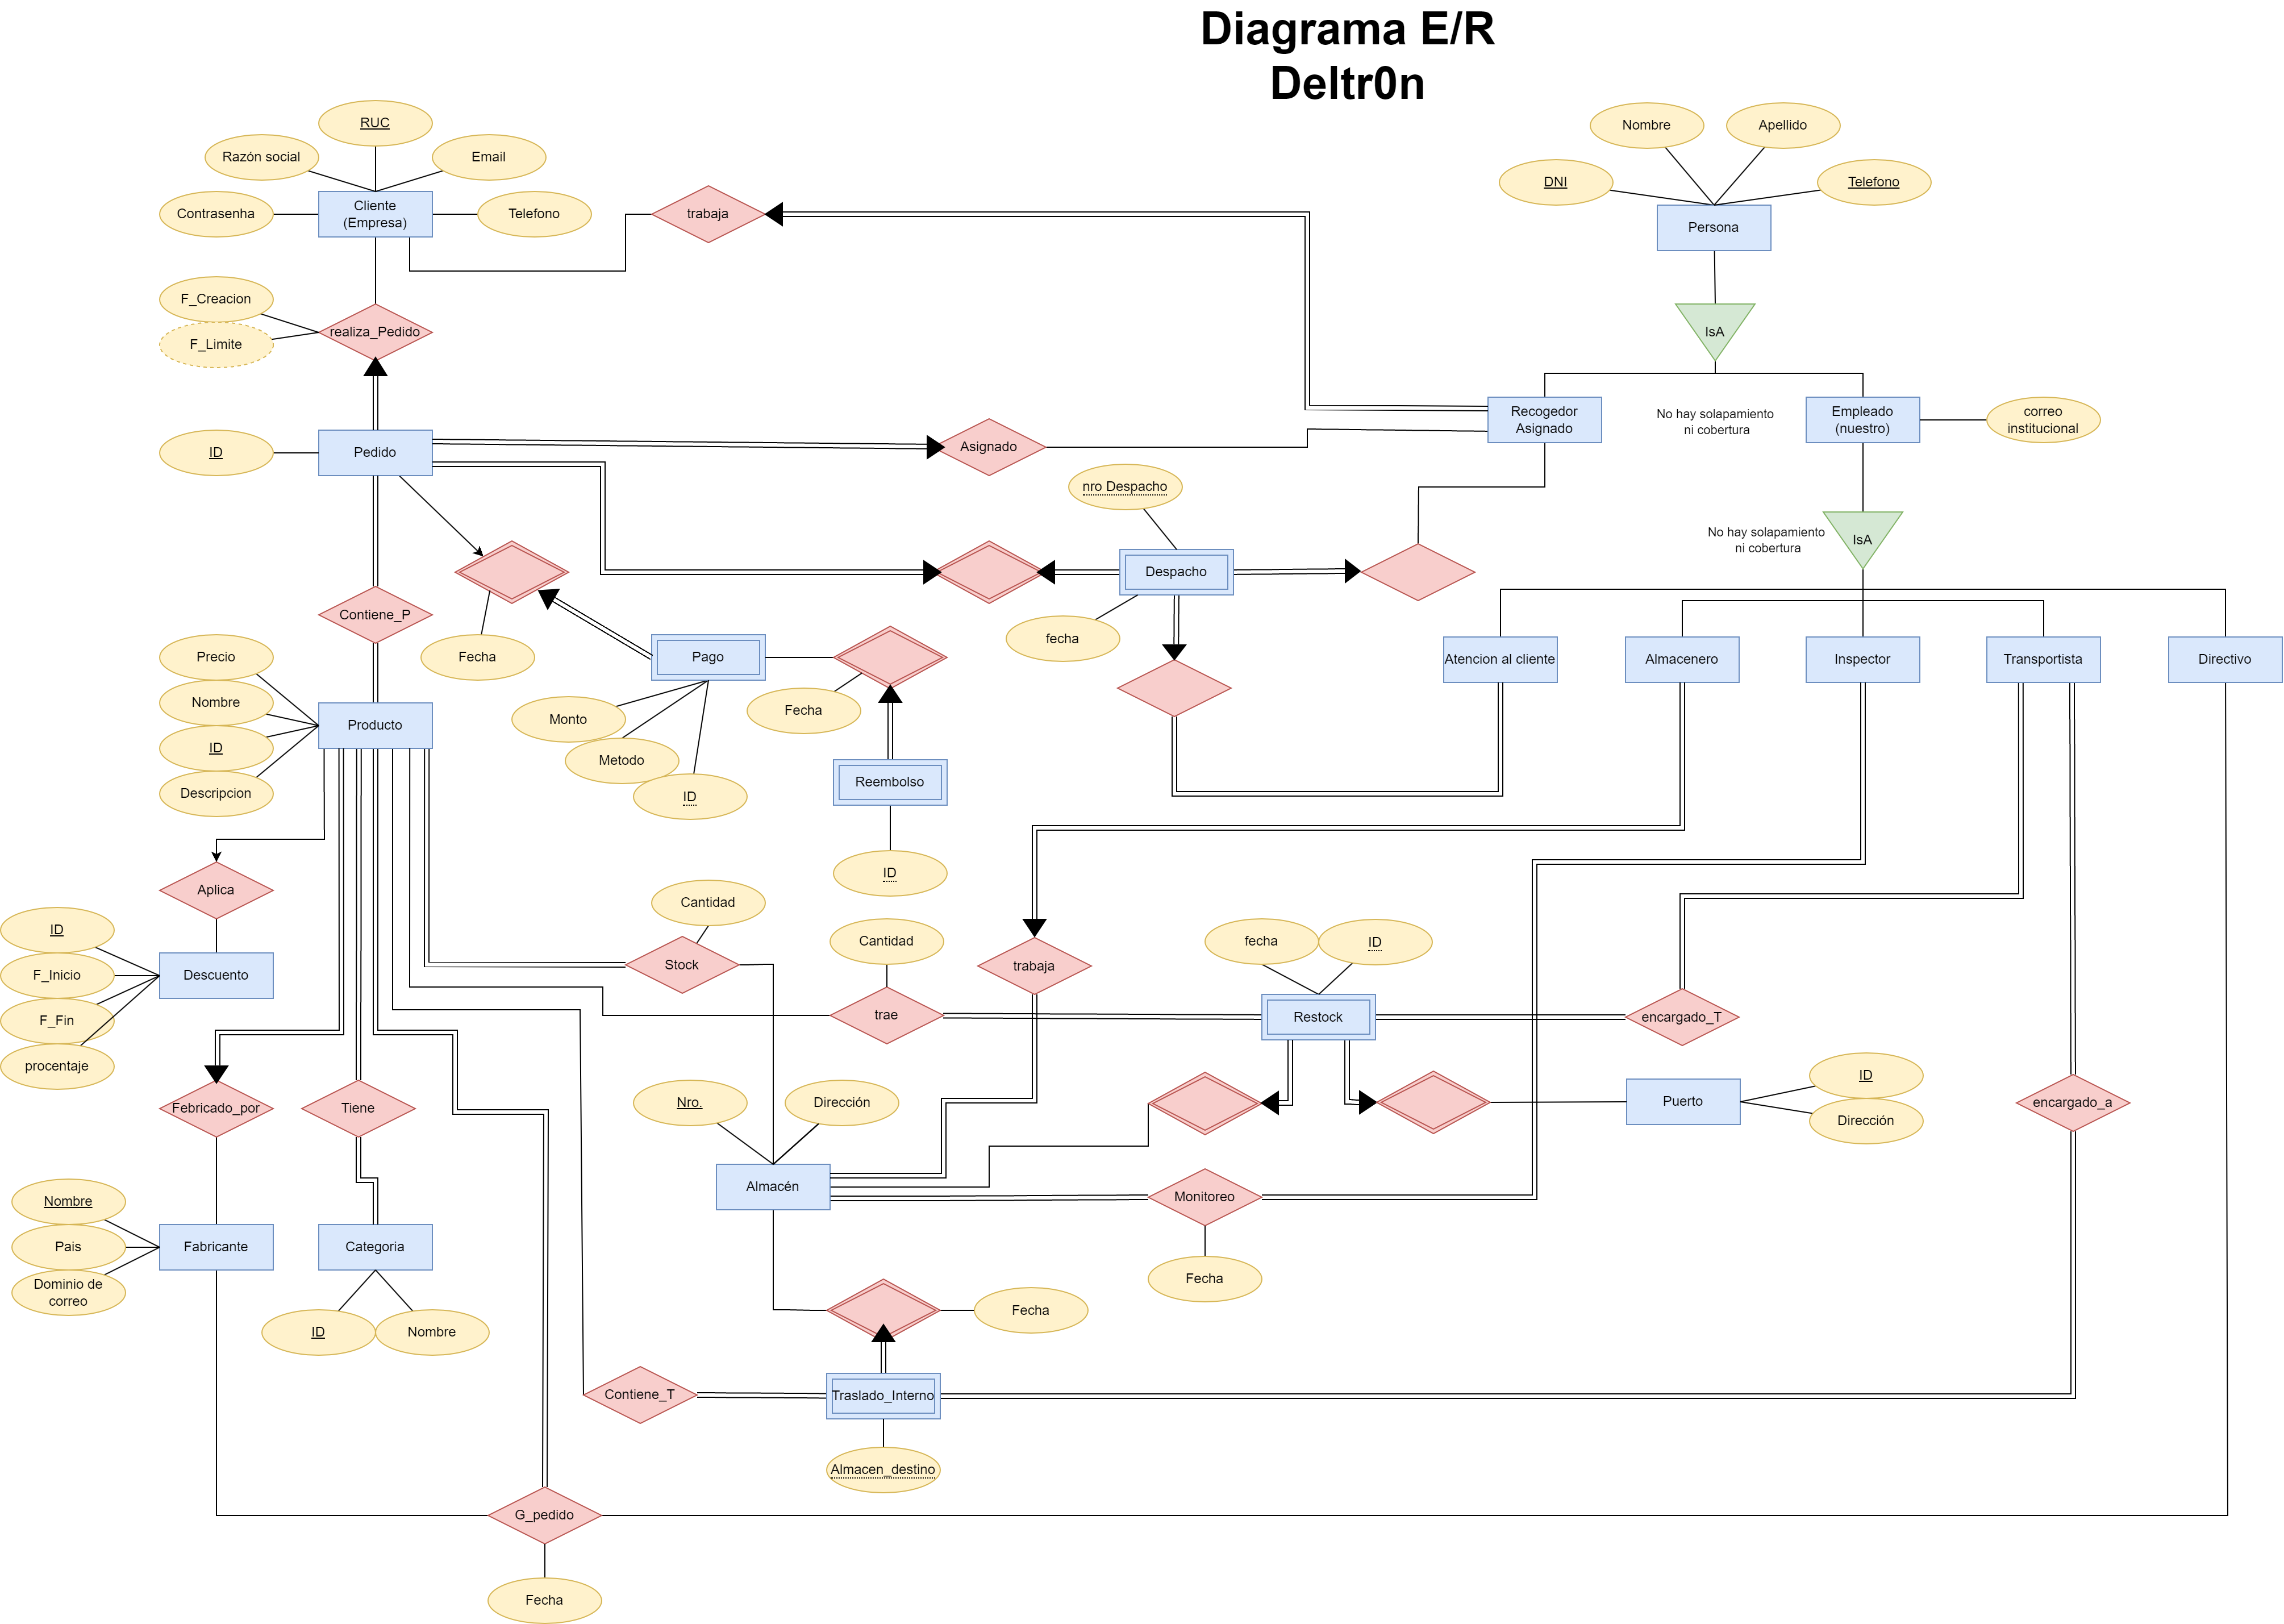
\includegraphics[width=1\textwidth]{./images/DER.png}



chapter ANEXOS (end)







\end{document}
